Astronomical surveys play an important role in developing scientific knowledge of the universe. 
The raw data in the form of telescope images are the primary source of information about the universe beyond our solar system. 
Often, the information in the raw data is consolidated into catalogs. 
Catalogs record light sources as stars, galaxies, or other objects; 
they also list their physical parameters such as flux, color, and morphology. 
In many cases, these catalogs are the starting point for downstream analyses of astronomical images.
For example, the Argonaut map which maps the 3D distribution of interstellar dust is based on the fluxes and colors of stars~\cite{Green_2019_argonaut}. 
Spatial distributions of galaxies have been used to validate theoretical models of dark matter and dark energy~\cite{Eisenstein_2005_darkmatter}. 

\jeff{
Some of the text below may be useful in the introduction. It explains the challenge in terms statisticians are more likely to connect with.
I haven't published it elsewhere, so feel free to include any parts verbatim if they are useful.

\textit{
Light source separation is challenging for several reasons.
First, it is an unsupervised problem with a sample size of one: there is not labeled data with known ground truth, and there is only one night sky, which is imaged many times.
Second, many stars and galaxies too faint to be unambiguously resolved. For these light sources, providing calibrated uncertainty estimates of our predictions is as important as making accurate predictions.
Third, many stars and galaxies overlap with other light sources---as many as 68\% of galaxies are expected to overlap with others in upcoming LSST survey.
As telescopes improve, even more galaxies will appear to overlap.
Fourth, the scale of the data is immense by any standard. The upcoming LSST survey, scheduled to begin data collection in 2022, is expected to produce 50 petabytes of astronomical images over its lifetime.
}
}

Our method considers applications where all sources are well-modeled as points without spatial extent. Estimation of location, fluxes, and color is the primary goal.
Point sources are good models for surveys where the primary objects studied are stars, such as DECam~\cite{Schlafly_2018_DECam}, which imaged the center of our own Milky Way. 
On the other hand, WISE~\cite{Wright_2010_WISESurvey} used point source models for cataloging because its telescope resolution and the density of light sources did not allow for differentiation between stars and galaxies. 

In this paper, we test our method on the globular cluster M2 imaged by the Sloan Digital Sky Survey (SDSS). 
Understanding these starfields is of scientific interest per se.
The distribution of colors and fluxes in crowded starfields 
can be used to estimate the age 
of the starfield, which in turn lower bounds the 
age of the universe~\cite{Isochrome_fitting}. 

% \begin{wrapfigure}{r}{0.5\textwidth}
%   \centering
%     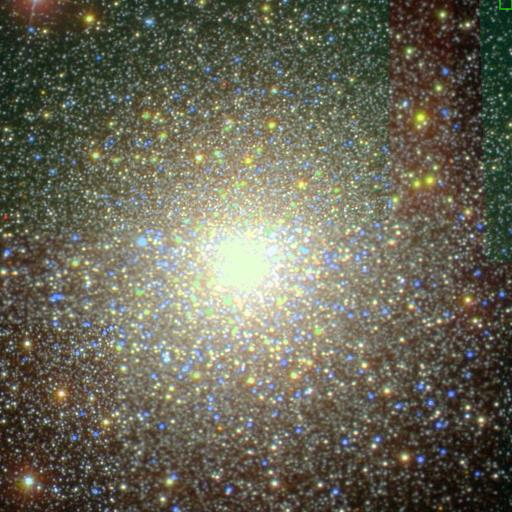
\includegraphics[width=0.3\textwidth]{figures/m2.png}
%   \caption{The globular cluster M2 as imaged by SDSS. }
% \end{wrapfigure}

\begin{figure}[!tb]
  \centering
    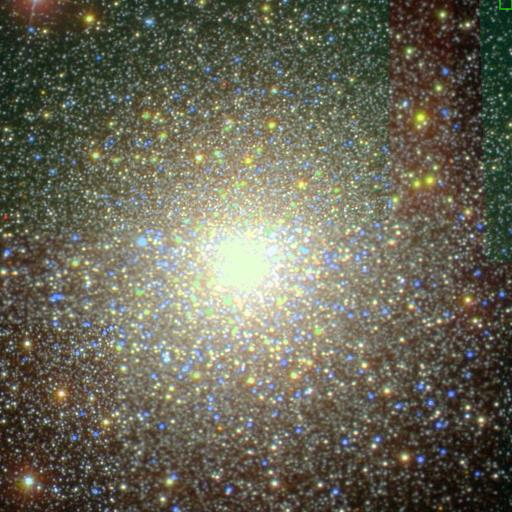
\includegraphics[width=0.3\textwidth]{figures/m2.png}
  \caption{The globular cluster M2 as imaged by SDSS. }
\end{figure}

For all the aforementioned applications, a key obstacle 
in catalog construction is the {\itshape blending} of light sources: in crowded fields, sources are no longer well-separated, and peak intensities may correspond to multiple sources. An algorithm producing a catalog should be able to reliably {\itshape deblend} the peak intensity, that is, distinguish whether the peak corresponds to one light source or 
multiple light sources. When the two cases are nearly unidentifiable from the data, the algorithm should 
report calibrated uncertainties. As telescopes improve and peer deeper into space, most images from future surveys will be in the crowded field regime. 
For example, \cite{Bosch_2017_LSST} estimates that in the Large Synoptic Survey Telescope (LSST), 68\% of the light sources will be blended. Therefore, developing a method to produce reliable catalogs even in cases of significant source blending will be important for advancing astronomical research. 

\subsection{From algorithmic pipelines to probabilistic cataloging}

Traditionally, most cataloging has been done using purely algorithmic pipelines, with steps involving locating the the brightest peaks, estimating fluxes, subtracting out the estimated light source, and repeating. 
Most of these pipelines are not designed for crowded starfields.
In fact, the default SDSS cataloging pipeline, called PHOTO~\cite{lupton2001sdss}, failed to 
produce a catalog on 
the globular cluster M2~\cite{Portillo_2017}. 
Not only do these pipelines fail in the crowded field
regime, but they also do not produce statistically calibrated error estimates that propagate 
uncertainties accumulating in each step of the pipeline. 

Previous work in \cite{Brewer_2013, Portillo_2017, Feder_2019}
propose {\itshape probabilistic} cataloging.
They propose a statistical model consisting of a likelihood for the observed image and a prior distribution over possible catalogs. Instead of deriving a single catalog, they produce a Bayesian posterior distribution over the set of all possible catalogs. 
Each sample from the posterior is a catalog; that is, posterior samples are tables, potentially of varying length, consisting of stellar locations, fluxes, and colors. 
Uncertainties are fully quantified by the posterior distribution. 
For example, in an image with an ambiguously blended bright peak, some catalogs drawn from the posterior would contain multiple dim sources while others would contain one bright source. 
The relative weight the posterior distribution places on one explanation over another represents the statistical confidence in that explanation. 
Moreover, a distribution over the set of all catalogs induces a distribution on any estimate derived from a catalog. Therefore, uncertainties can be fully propagated to downstream analyses.  

In previous work on probabilistic cataloging, the posterior was computed using Markov chain Monte Carlo (MCMC).
\cite{Portillo_2017, Feder_2019} refer to their method as PCAT, short for ``Probabilistic CATaloging."\footnote{
We use ``probabilistic cataloging'' to refer to any method that produces a Bayesian posterior over possible catalogs, whereas ``PCAT" refers specifically the the MCMC procedure in~\cite{Portillo_2017, Feder_2019}. }
However, the computational cost of MCMC is prohibitive for large-scale astronomical surveys. 
PCAT required 30 minutes to process a $100\times 100$ pixel subimage of the globular cluster M2~\cite{Feder_2019}, roughly a $0.3\times0.3$ arcsecond patch of the sky.
For comparison, in one night SDSS scans a region of size on the order of $10 \times 1000$ arcminutes. Extrapolating the reported 30min runtime, PCAT would take about two months to process one night's data collection.
Future surveys will only get larger. 
The upcoming LSST survey, scheduled to begin data collection in 2022, is expected to produce 50 petabytes of astronomical images over its lifetime---approximately 15 terabytes nightly~\cite{LSST_about}. 
The size of the data is immense by any standard, and an important challenge is to develop inference methods that scale to these large astronomical surveys. 

\subsection{Variational inference and neural networks}
As an alternative to MCMC, our method constructs an approximate posterior using variational inference~\cite{Blei_2017_vi_review,Jordan_intro_vi, Wainwrite_graph_models_vi}.
With variational inference (VI), we propose a family of distributions and use numerical optimization to find the distribution 
in the proposed family that is closest 
in KL divergence to the exact posterior. 
With a sufficiently constrained family of distributions, the VI optimization problem can be orders of magnitude faster than MCMC. 

We are not the first to propose a VI procedure
that scales Bayesian inference to the terabytes of data collected by astronomical surveys. 
\cite{regier2019_celeste} also employed 
VI, and with the help of a 650,000 core supercomputer, they constructed a catalog of the entire Sloan Digital Sky Survey based on Bayesian inference. 
% \jeff{The program isn't called Celeste in \cite{regier2019_celeste}. You might just keep citing the paper rather than calling the program Celeste.}

However \cite{regier2019_celeste} has two limitations. The first is that the number of light sources in a given image is treated as known and fixed in their statistical model; thus, it had to be set by a preprocessing routine. In this work, the number of sources is assumed to be unknown and modeled as a latent variable. 
This results in a transdimensional latent variable space 
since the posterior is defined over the set of all catalogs, and the number of sources in a catalog is unknown and random.
Previous work on probabilistic cataloging employed reversible jump MCMC~\cite{Green95reversiblejump} to sample transdimensional catalogs. In RJ-MCMC, auxiliary variables are added to encode the ``birth" of new sources 
or the ``death" of existing sources in the Markov chain. 
Our challenge in VI is to construct a family of distributions on this transdimensional space.
Section~\ref{sec:var_distr} discusses the construction: 
a variational distribution is defined over catalogs of all possible size, that is, a triangular array of latent locations and fluxes; 
a distribution on the triangular array then induces a distribution on the set of all catalogs.

Secondly, in~\cite{regier2019_celeste}, numerical optimization had to be re-run for every new collection of images. 
In contrast, our method employs {\itshape amortized} variational inference, where a neural network is trained to map input images to a variational distribution.
After a one-time cost to train the neural network, inference 
on a new image requires just a single forward pass.
In the architecture detailed in Section~\ref{sec:nn_archetecture}, the forward pass on 
a $100 \times 100$ pixel subimage of M2 takes $\approx 0.2$ seconds (cf. 30 minutes with MCMC). 
Moreover, neural networks can efficiently evaluate batches of images in parallel on a GPU. 
This amortization is advantageous for scaling up inference to large astronomical surveys.
% \jeff{The most serious limitations of~\cite{regier2019_celeste} are that 1) the number of light sources is set by a preprocessing routine and fixed, 2) the variational distribution for some random variables is a point mass, including location.
% This paper fixes both problems by using stochastic optimization, whereas~\cite{regier2019_celeste} used deterministic optimization.
% Stochastic optimization is in general slower than deterministic optimization, but in this paper we get a speedup by using amortized inference.
% In addition to greater speed, amortized inference may be better at nonconvex optimization: by learning a policy from many examples we learn a policy for avoiding shallow local minima. No carefully hand-tuned initialization scheme is needed.
% }
% \bryan{Wait, could you explain a bit more about how stochastic optimization helps us avoid (1) and (2)? 
% I agree that these two issues should be mentioned, since
% simply saying "we are faster" than this other VI procedure might not be enough motivation for this work. }

Neural networks have seen great success on image classification tasks~\cite{imagenet2015}, and our method leverages their predictive power and computational efficiency for detecting and deblending stars in telescope images.
However, our neural network goes beyond returning a class label, such as whether the image is classified to be of one object or another. 
Instead, the neural network specifies an approximate Bayesian posterior in the context of a well-defined statistical model. 

\subsection{The wake-sleep algorithm}

In traditional variational inference, the neural network is trained to minimize the ``reverse" KL between the variational distribution $q$ and the true posterior $p$, defined as the $q$-weighted average difference between $\log q$ and $\log p$. 

Our method instead trains the neural network using the ``forward" KL divergence, which weights the difference between $\log q$ and $\log p$ by $p$. Procedurally, to minimize this loss, catalogs are sampled from the prior distribution along with corresponding images from the likelihood model. 
The neural network is trained to map sampled images to distributions that place probability mass on their corresponding catalogs. 
We find that in our application, optimizing the forward KL produces more reliable approximate posteriors than optimizing the traditional reverse KL. 
In particular, by taking advantage of complete data -- the sampled images and their corresponding catalogs -- our method is able to avoid shallow local minima where the approximate posterior returned by the neural network is far from the true posterior in KL divergence. 

Minimizing the forward KL is known as the ``sleep" phase in the wake-sleep algorithm, since this phase employs sampled data from the statistical model. 
In the ``wake" phase of the algorithm, the variational distribution is fixed, and model parameters are optimized using observed data. 
This is equivalent to the M-step in variational EM~\cite{Jordan_intro_vi, neal2000varem, Beal2002varem}.
The wake phase ensures that the statistical model matches as closely as possible to the real data generating process. 
In this application, the wake phase is used to estimate the point spread function and the sky background in telescope images. 

In summary, our method takes advantage of the flexibility of neural networks to construct a mapping from telescope images to an approximate Bayesian posterior on the set of all catalogs. 
The neural network is trained using complete data 
in which both the image and the catalog are known. 
In our application, this training procedure produces a mapping that avoids shallow local minima in a difficult nonconvex optimization problem. 
Model parameters such as the point spread function are also tuned. 

We call our method to produce probabilistic catalogs {\itshape StarNet.}
Section 5 compares the catalog obtained from StarNet with the MCMC-based cataloger PCAT;
it also compares with traditional cataloging approaches.

% However, in addition to greater speed, amortized inference may be better at nonconvex optimization: by learning a policy from many examples we learn a policy for avoiding shallow local minima. 



% In particular, the usual stochastic gradients of the reverse KL 
% were too high-variance to be used in in our application; 
% in contrast, low-variance stochastic gradients of the forward KL are computationally cheap to compute. 


% low-variance stochastic gradients of the forward KL are much cheaper to compute than stochastic gradients of the reverse KL. Moreover, we hypothesize that amortized inference may be better at nonconvex optimization: by learning a policy from many examples we learn a policy for avoiding shallow local minima. 






% The neural network outputs are not simply ``labels" for the input image 






% In traditional variational inference, the divergence between 
% the variational posterior $q$ and the true posterior $p$ is 
% measured by the ``reverse" KL divergence, defined as the 
% $q$-weighted average difference between $\log q$ and $\log p$. In other words, the reverse KL divergence
% is defined by an expectation with integrating distribution $q$. 

% In simple models, for example when $p$ and $q$ are appropriate classes of exponential families, 
% the expectation over $q$ can be written explicitly as a function of the parameters of $q$. Therefore, the minimizer of the KL can be solved either in closed form or by employing deterministic optimization~\cite{Blei_2017_vi_review}. 

% In our setting of amortized variational inference, the parameters of $q$ are neural network weights. When analytic expectations are unavailable, as in our case, 
% sampling methods have been employed in conjunction with modern auto-differentiation tools to compute stochastic gradients. Optimization is done with stochastic gradient descent. Examples include black-box variational inference (BBVI)~\cite{ranganath2013black} 
% and automatic-differentiation variational inference (ADVI)~\cite{kucukelbir2016automatic}. The latter 
% is closely related to the reparameterization trick \cite{kingma2013autoencoding, rezende2014stochastic} proposed to train deep generative models using the KL objective. 
% These approaches all sample latent variables from $q$ and produce an unbiased estimate 
% for the gradient of the KL. 

% However, the reparameterization trick does not apply when any latent variables are discrete, in our case, the number of stars. The REINFORCE estimator~\cite{Williams1992reinforce}, which BBVI adapts, produces an unbiased stochastic gradient for both continuous and discrete latent variables. However, the REINFORCE estimator often suffers from high variance in practice, and so the resulting stochastic optimization is slow. 

% The key difficulty is that the the objective function is 
% an expectation with integrating distribution on $q$, the  distribution to be optimized. To avoid this issue, the {\itshape wake-sleep} algorithm considers the ``forward" KL divergence, defined as the
% $p$-weighted average difference between $\log p$ and $\log q$;  in other words, the expectation is taken over $p$. To make the forward KL divergence tractable, a second average is taken over possible data. In other words, the neural network is trained so that {\itshape on average over possible input images $x$}, the 
% variational distribution returned by the neural network is close to the true posterior in forward KL divergence. 

% Low-variance stochastic gradients are easy to compute using the wake-sleep algorithm, and we show that these low-variance gradients result in faster optimization than using the REINFORCE gradient estimator. 
% However, in addition to greater speed, amortized inference may be better at nonconvex optimization: by learning a policy from many examples we learn a policy for avoiding shallow local minima. 



% In simple models, for example when both $p$ and $q$ are related exponential families, the expectation can be written explicitly as a function of the parameters of $q$~\cite{Blei_2017_vi_review}. Therefore, the KL can be minimized either in closed form, or by using deterministic optimization. However, in our case, the parameters of $q$ are neural network weights. In this setting, ~\cite{rezende2014stochastic,kingma2013autoencoding} propose 
% stochastic optimization, where an unbiased gradient of the KL divergence is computed from samples of $q$. 





% One limitation of neural networks is the large amount of data needed for training.
% In astronomy, knowledge of the physical system  often give rise to reasonably realistic simulators for data. For example, simulators were used in \cite{Lanusse_2017_cmudeeplens} trained neural networks to detect Einstein rings, 
% a rare object found in astronomical surveys and used to study dark matter; the neural network in \cite{Hezaveh_2017_nn_lensing_nature} also returned
% morphological parameters for each Einstein ring. 
% In both cases, because the training data was generated from a simulator, the ground truth labels (ring exists or not; the ring morphology) are known. The network is trained in a supervised fashion. Using simulated data is especially useful because the network can be trained on essentially unlimited data -- the bottleneck is the limit on computational resources, not the availability of training data. 

% In our work, we also make use of simulated data to train our neural network. However, we introduce the simulated data in the context of a statistical model. We do so using the wake-sleep algorithm~\cite{Hinton1995wake_sleep}. 
% The neural network outputs are not simply ``labels" for the input image; rather, we are able to interpret the output as specifying an approximate Bayesian posterior in the context of a well-defined statistical model. 

% In summary, we leverage the predictive power and computational efficiency of neural networks to do 
% inference in the framework of a statistical model. 
% We also employ simulated data in our training procedure in a statistically principled way. In Section~\ref{sec:results}, we compare the catalog obtained from our variational posterior with the catalog derived from MCMC; we also compare with traditional cataloging approaches.  

% detect Einstein rings; \cite{Hezaveh_2017_nn_lensing_nature} used
% neural networks to infer morphological characteristics of the Einstein rings; 
% in the context of deblending, 
% \cite{Reiman_2019_gans_deblend} used 
% GANS to separate two overlapping galaxies. 

% Several factors contribute to the success of neural networks. Firstly, neural networks are computationally efficient; multiple images can be easily evaluated in parallel on a GPU.
% Secondly, a well-trained neural network is able to generalize beyond the data on which is was trained. This combined with computational efficiency is extremely beneficial for sky surveys: after training a neural network on a subset of the survey, the remaining images in the survey can be evaluated quickly in batches using only forward-passes through the network. 

% In this paper, we combine the flexibility of neural networks with a formal statistical model. This enables the neural network output to be interpreted in a statistically principled way: the output of our neural network will be a distribution that approximates the Bayesian posterior.

% Secondly, we train the neural network using {\itshape wake-sleep} training. This allows our neural network to be trained using unlimited simulated data. Using simulated data to train neural networks is common practice is astronomy (see for example~\cite{Lanusse_2017_cmudeeplens, huang2019finding}). However, we also make the connection with a formal statistical model 
% and introduce the simulated data in a principled way. TODO: yikes ... this paragraph is terrible and needs work. 

% In Section~\ref{sec:gen_model} we introduce 
% the generative model. Section~\ref{sec:var_inference} details the variational distribution and discuss training of the neural network. Section~\ref{sec:related_work} makes connections with previous cataloging software. In Section~\ref{sec:results}, we compare 
% our variational inference procedure with MCMC as well as more traditional cataloging software pipelines. Section 6 concludes. 

